\chapter{Discussion} \label{chap:experimental}
% -------------------------
%% QUOTE
\vspace*{\fill}
\epigraph{The aim of argument, or of discussion, should not be victory, but progress.}%
{\textit{"The Notebooks of Joseph Joubert". Translated by Paul Auster.}\\ \textsc{Joseph Joubert}}
\clearpage{\thispagestyle{empty}\cleardoublepage}
%%
%% Body of the chapter
%%%%%%%%%%%%%%%%%%%%%%
\section{Preparation of nanogels based on polyelectrolyte complexes}
A limited number of experiments have been done in order to test the possibility of delaying gel formation by incorporation of the cross-linker in PEC. Tests with PECs based on published Texas A\&M technology showed that it was possible to delay gelation for in the order of 20 days when the sample was aged at 50~\celsius. At 80~\celsius~ the gelation was much faster, comparable to systems cross-linked with \ce{Cr^3+}. Fast gelation was observed also for reduced amounts of \ce{Cr^3+} in the PEC.

When the PEC was modified by changing the original polycation with amide POSS and with use of PVS as polyanion delayed gelation for in the order of 20 days and possible longer for aging at 80~\celsius. This delay in gelling appeared to be independent of polymer concentration and the concentration and composition of the PECs. The results indicate that the concept of making PEC with amide POSS as polycation may be viable. However, more experiments must be done to optimise the PEC. Other polyanions such as DS should also be tested with amine POSS. The transport properties of PECs in porous media has not been tested.

Going from the Texas A\&M technology PECs to the amine POSS/PVS PEC reduces the number of components by one. This can possibly make the PECs more robust for transport in porous media where chromatographic separation of the constituents may occur. However, other factors may also govern the stability of PEC particles when transported in porous media.

Retarded gelling obtained with a single cross-linker is possibly the best solution if a suitable system can be developed. The use of lactamide POSS appears to be promising. The requirement to retarded gelation will depend on how long into a reservoir a gel zone must be placed in order to obtain the desired water diversion. Then factors like initial viscosity, viscosity vs. time developments, shear tinning and allowable injection pressures becomes important for defining the properties of the fluid system.

The prepared polymer/PEC solutions have been based on high molecular weights polymers giving relatively high initial viscosities (although measured at 20~\celsius~ and shear rates of 54.6$^{-1}$ or lower). The lactamide POSS system was developed with a polymer that gave a significantly lower viscosity, although a higher polymer concentration was used. For practical applications (costs and logistics) it will be desirable to formulate a system with as little as possible use of chemicals still giving a viscosity increase after injection sufficient to divert water when placed in a reservoir. Thus, a significant development work still will be needed to formulate an optimal system.


\section{Core flooding experiments for transport in porous media}
The absolute permeabilities of the cores used in the flooding experiments were determined before and after the experiments with nanoparticle and/or polymer injection. The residual resistance factor is defined by the ratio of initial and final permeability for the experiment. The results are shown in Figure \ref{fig:ipvRet1}. In total three experiments were conducted with nanoparticles and Berea sandstone but only two determinations of residual resistance factors were done (Berea NP1 and Berea NP2).

As seen in Figure \ref{cht:rrf} contact with only nanoparticles did not change the permeability significantly. Contact with polymer reduced the permeability, especially for the Bentheimer core. The effect of adding nanoparticles to the polymer had different effects on the two different core materials. The decrease in the residual resistance factor for Bentheimer questions the value obtained with only polymer.

Figure \ref{cht:polAds} shows the results from the determination of polymer adsorption. As expected, the adsorption was much less for the almost clean high permeability Bentheimer sandstone compared to Berea sandstones that had lower permeability and most likely significantly higher specific surface area (m2/g rock) It is known that Berea also contain significant amounts of clay minerals.

\begin{figure}[p]
    \centering
    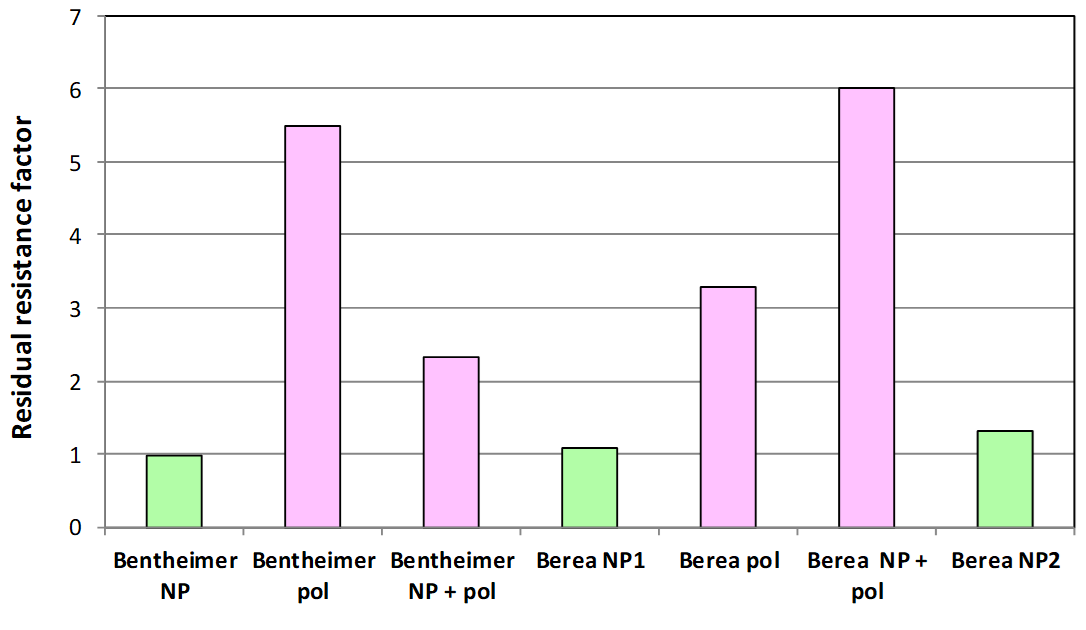
\includegraphics[width=\textwidth]{img/cht/rrf.png}
    \caption{Residual resistance factors.}
    \label{cht:rrf}
\end{figure}

\begin{figure}[p]
    \centering
    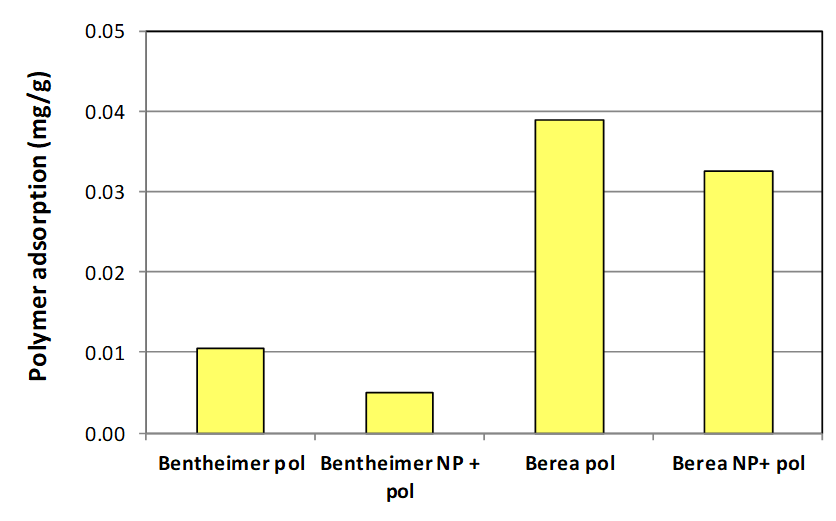
\includegraphics[width=\textwidth]{img/cht/polAds.png}
    \caption{Residual resistance factors.}
    \label{cht:polAds}
\end{figure}

The inaccessible pore volumes determined are shown in Figure \ref{cht:ipvPol}. For Bentheimer sandstone the IPVs were low and close to the same with and without nanoparticles in the injected fluid. For Berea, the IPV decreased when nanoparticles were added. 

The IPV is a measure for the fraction of the pores that were too small for the large polymer molecules to enter. It is difficult to understand how nanoparticles affected the polymer to enter smaller pores unless the polymer molecules curled up and got lower effective particle diameters in their presence. However, the differential pressure towards the end of stages 1 and 3 were higher with nanoparticles, but not more than the different rates used in the two experiments should give (cf. Figure \ref{cht:injexp5ber1} and Figure \ref{cht:injexp6ber1}). 

\begin{figure}[p]
    \centering
    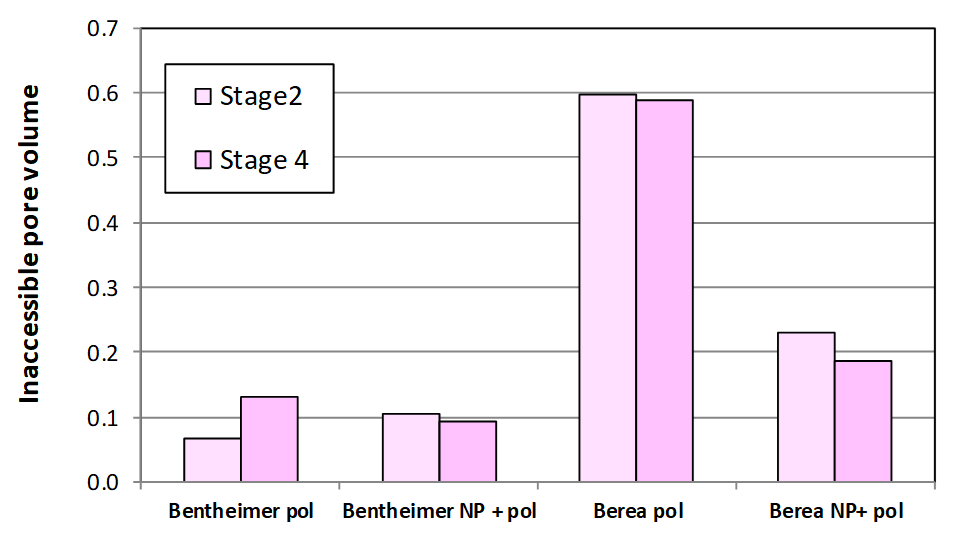
\includegraphics[width=\textwidth]{img/cht/ipvPol.png}
    \caption{Residual resistance factors.}
    \label{cht:ipvPol}
\end{figure}

IPVs were also calculated for nanoparticles. Also in this case IPVs were calculated based on the integral under the production curves as shown in Figure \ref{fig:ipvRet2}. In all mass balance equations, it was assumed that the nanoparticles entered the whole pore volume. and the IPVs thus has a different physical meaning than for polymer. As seen in Figure \ref{cht:ipvNP} most of the IPVs are negative. A negative IPV means that more than one pore volume of nanoparticles was produced during SSW flooding, \textit{i.e.}, some of the nanoparticles retained during injection was released during the subsequent SSW flooding.

For some experiments, the IPV s were calculated based on both refractive index and UV detector responses, and different interpretations of the detector response. The values shown in Figure \ref{cht:ipvNP} are average values and the standard deviations are indicated by arrow bars. The results for Berea NP1 are averages for the experiments conducted in January and February 2016, whereas Berea NP2 are average results for the experiment carried out in June 2016.

\begin{figure}[p]
    \centering
    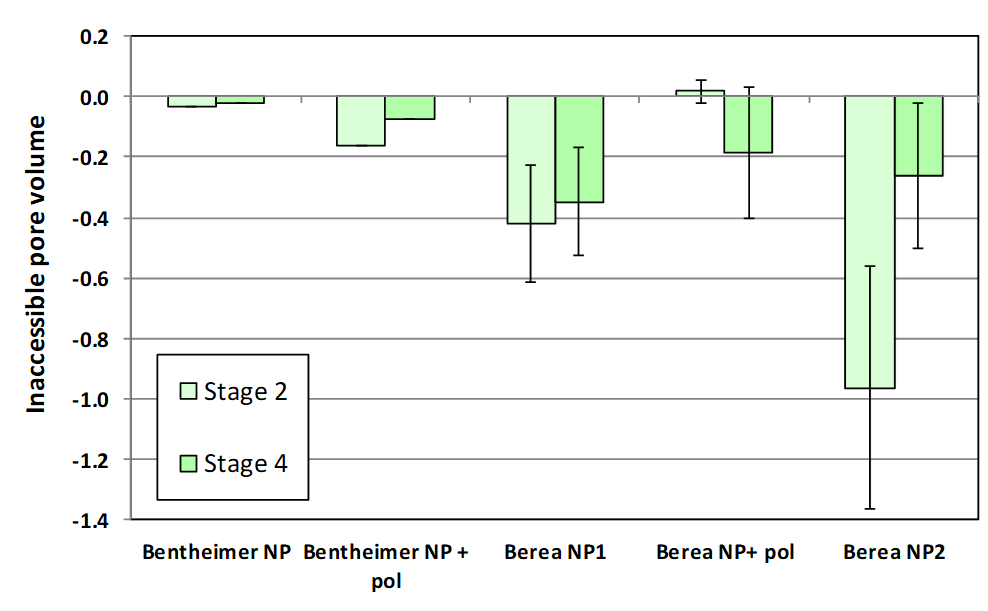
\includegraphics[width=\textwidth]{img/cht/ipvNP.png}
    \caption{Residual resistance factors.}
    \label{cht:ipvNP} % 5.23
\end{figure}

As seen in Figure \ref{cht:ipvNP}, the IPV values for nanoparticles were negative, but low for Bentheimer sandstone. For Berea sandstone, the IPVs were much lower and the uncertainty in the results are significant. 

Figure \ref{cht:retentionMech} shows the retention of nanoparticles and mechanical entrapment of polymer during all experiments. For nanoparticles in Berea sandstone the average values shown in Figure \ref{cht:retentionBer} are used. For other experiments where more than one datasets exist average values are also used. The two groups of bars to the left in the figure are for experiments where only nanoparticles or only polymer was injected. The two groups to the right are for injection of mixtures of nanoparticles and polymer.

\begin{figure}[h]
    \centering
    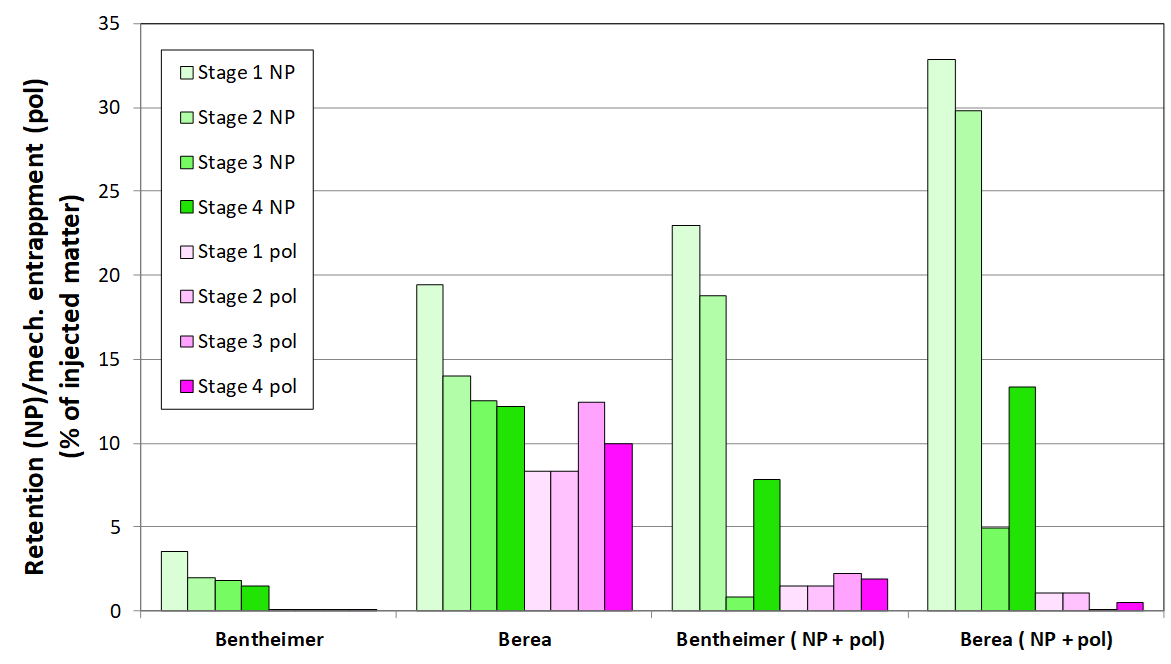
\includegraphics[width=\textwidth]{img/cht/retentionMech.png}
    \caption{Residual resistance factors.}
    \label{cht:retentionMech} % 5.24
\end{figure}

For polymer, the mechanical retention was low in all experiments except for injection of only polymer in Berea sandstone. No errors have been detected in the data processing and ta mechanical retention in the order of 10 \% appears to be real. As already discussed, it is curious that the mechanical retention is close to zero with added nanoparticles. 

The retention of only nanoparticles in Berea is associated with large uncertainty, in the order of ± 10 \% of injected matter (cf. Figure \ref{cht:retentionBer}). The large retention of nanoparticles during injection of the mixtures on stages 1 and 2 can possibly be due to detector response problems. 

\FloatBarrier
\section{Experiments with in situ gelling}
Table \ref{tab:porPermAge} summarizes the initial absolute permeabilities of the cores used in the experiments, the permeabilities measured with SSW injection after the aging and the residual resistance factors (RRF), \textit{i.e.} the ratio between the two permeabilities. The resistance factor determined after 7 days of aging was not much higher than the corresponding factor determined for polymer injection into Bentheimer sandstone, \textit{cf.} Figure \ref{cht:rrf}. As shown by Table \ref{tab:porPermAge}, the residual resistance factors increased with longer aging times for the first three experiments.
%TAB
\begin{table}
\footnotesize
\centering
\caption{Porosities, initial and final permeabilities and residual resistance factor for various aging times.}
\label{tab:porPermAge} % 5.12
\begin{tabular}{c l l l l l } 
\toprule
\textbf{Exp. no.} & \textbf{Porosity} & \textbf{Aging time} & \textbf{Abs. perm.} & \textbf{Residual perm.} & \textbf{RRF} \\ 
 & [fraction] & [days] & [mD] & [mD] & \\
\midrule 
1  & 0.221   &  7     & 2653     & 306      & 8.7    \\
2  & 0.221   & 23     & 2580     & 5.2      & 493      \\ 
3  & 0.221   & 66     & 2706     & 0.8    & 3230   \\ 
4  & NM* & Injectivity test & 2571    & -        & -      \\
5  & 0.224   & 53     & 2710     & 0.002        & 158000      \\
\bottomrule
* Not measured.
\end{tabular}
\end{table}

The injection phases for the nanoparticle/polymer solution are compared in Figure \ref{cht:gelexp_sum}. As seen the differential pressures across the viscometer tube were similar except for a slightly higher viscosity of the solution used in Experiment 5. In Experiment 3, parts of the bypass line was filled with the nanoparticle/polymer mixture, explaining the initial decline in the viscosity response. 

\begin{figure}[h!]
    \centering
    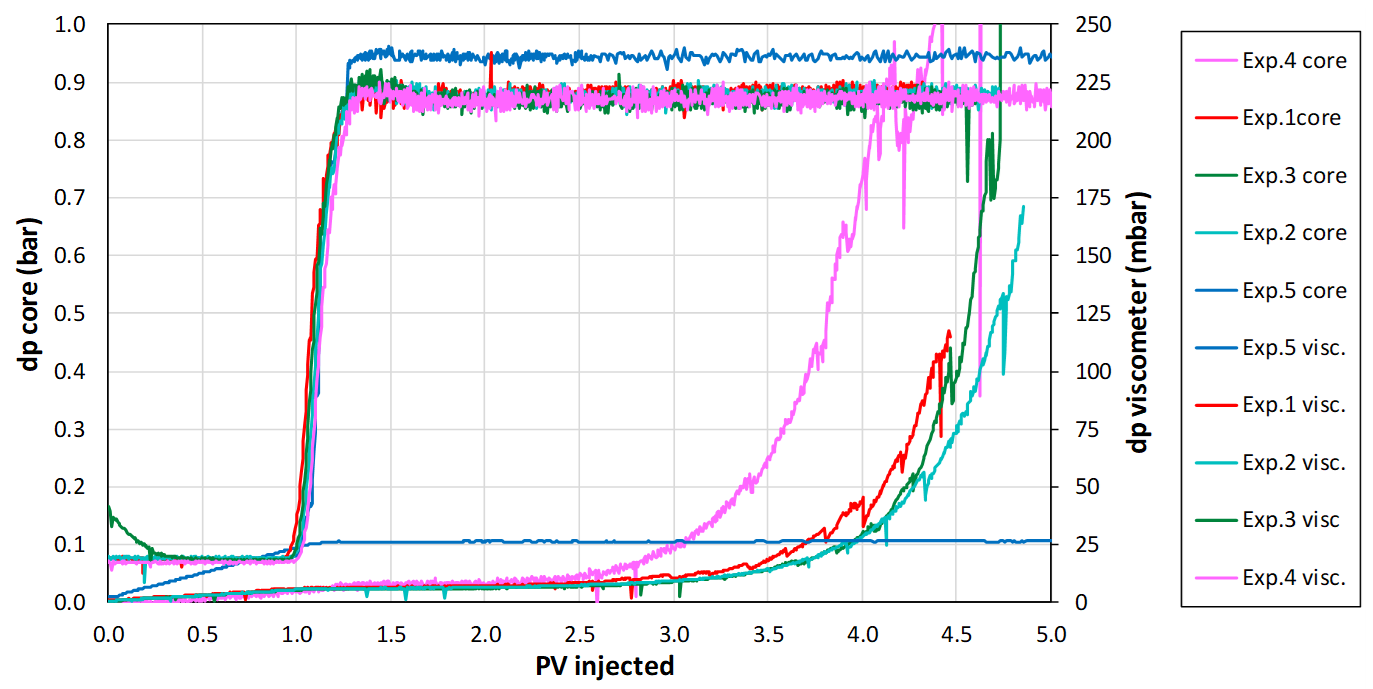
\includegraphics[width=\textwidth]{img/cht/gelexp_sum.png}
    \caption{Comparison of nanoparticle/polymer injection phases.}
    \label{cht:gelexp_sum} % 5.39
\end{figure}
 
The differential pressures over the core developed almost identical for the first 2.5 PVs injected. The rapid increase thereafter, developed in different, but quite similar manners. Pre-Filtering of the injected solution through a 500 mD core (Experiment 4) apparently gave a worse result compared to filtration through 8 \micro m membrane filters in Experiments 1 through 3.

If the presence of extended structures/particles in the solution was the cause of the injectivity problem, the use of finer filters could possibly alleviate the problem. In Experiment 5, the injected solution was filtered through 6 \micro m and then 3 \micro m filters. Likely more important, the pH of the injected solution was reduced to 7.2 which resulted in a clear solution before filtering. It was shown in section \ref{sec:phInSitu} that lowering of the pH removes visible precipitates from the nanoparticle/polymer solution. This removal of precipitates can have a direct impact on the injectivity. 

As can be seen in Figure \ref{cht:gelexp_sum}, the differential pressure across the core did not increase after breakthrough of the nanoparticle/polymer solution in Experiment 5, and it remained stable until all available solution was injected (15.3 PV). The improved treatment thus alleviated the injectivity problem seen in the first four experiments. After 53 days of aging at 80~\celsius, SSW was injected into the core at 27 bar differential pressure that corresponded to a pressure gradient of 135 bar/m. After 210 hours of SSW injection, no yield in the gel strength was observed. This result demonstrates that pH adjustment and improved filtering did not impair the gel strength.

The experiments with \textit{in situ} gelling have demonstrated that gel was formed in the porous medium. As expected the gel strength increased with increased gelling time. For gelling times in the order of 2 months strong gels were formed. 

In Experiment 3, the gel almost blocked the core with a pressure gradient of 135 bar/m for 9 days at 80~\celsius. In Experiment 5, the gel blocked the core during the entire test period of 45 days using the same pressure gradient and temperature. At the end of Experiment 5 the flow rate of SSW through the core was 0.23 ml/hr. 

\section{Oil recovery experiments}

The oil recovery experiments demonstrated that the wettability of the rock can have a significant effect on the oil recovery during SSW injection. For the water wet system, the oil recovery was poor, \textit{i.e.}, only 35.2 \% of the original oil in place. The neutral wet system behaved completely differently, as 81.9 \% of the oil originally in place was recovered. The addition of FN-nanoparticles did not affect the recovery in neither of the experiments.

\section{Numerical simulation}
Simulations using the developed 1D simulator show a good match to experiments on break through times for polymer and nanoparticles. Important effects such as IPV, adsorption, viscosity changes and trapping is hence accounted for. The simulator can, however, not take into account heterogeneities in the cores and the polymer and nanoparticle responses are seen to be piston like. To account for heterogeneities, expansion to 2D or 3D is required, this is shown by simulating simple heterogeneities using the ECLIPSE simulator. The effect of physical dispersion at the front and tail of the injected solution could be implemented with the use of a mixing parameter like in ECLIPSE, this should be considered in future versions. 

The functionality of gelling is modelled and simulations indicate correct behaviour in a large scale 1D model. To model field scale practical use of the system would require an extension of the simulator to 2D or 3D. All the main functionality has been developed in the 1D simulator and future extension to 2D and 3D is suggested to be performed within the MRST framework ( http://www.sintef.no/projectweb/mrst/ ).

The effect of increase in residual resistance factor after the effect of gelling has not been implemented in the current code, this should be considered for future versions.
